\section{Block Level Description}

\subsection{SPI/PSRBR}

\subsection{16-bit Kogge-Stone Adder}
\begin{table}[H]
\caption{Example table boolean expressions for combinatorial gates}
\centering
\begin{tabular}{cccc}
\toprule
Input & Function1 & Function2 & Output \\
\midrule
00 & 1 & 0& 1\\
01 & 0 & 0 & 1\\
10 & 0 & 0 & 1\\
11 & 1 & 0 & 1\\
\bottomrule
\label{tab:SPI}
\end{tabular}
\end{table}

\begin{figure}[H]
  \centering
  \captionsetup{justification=centering}
  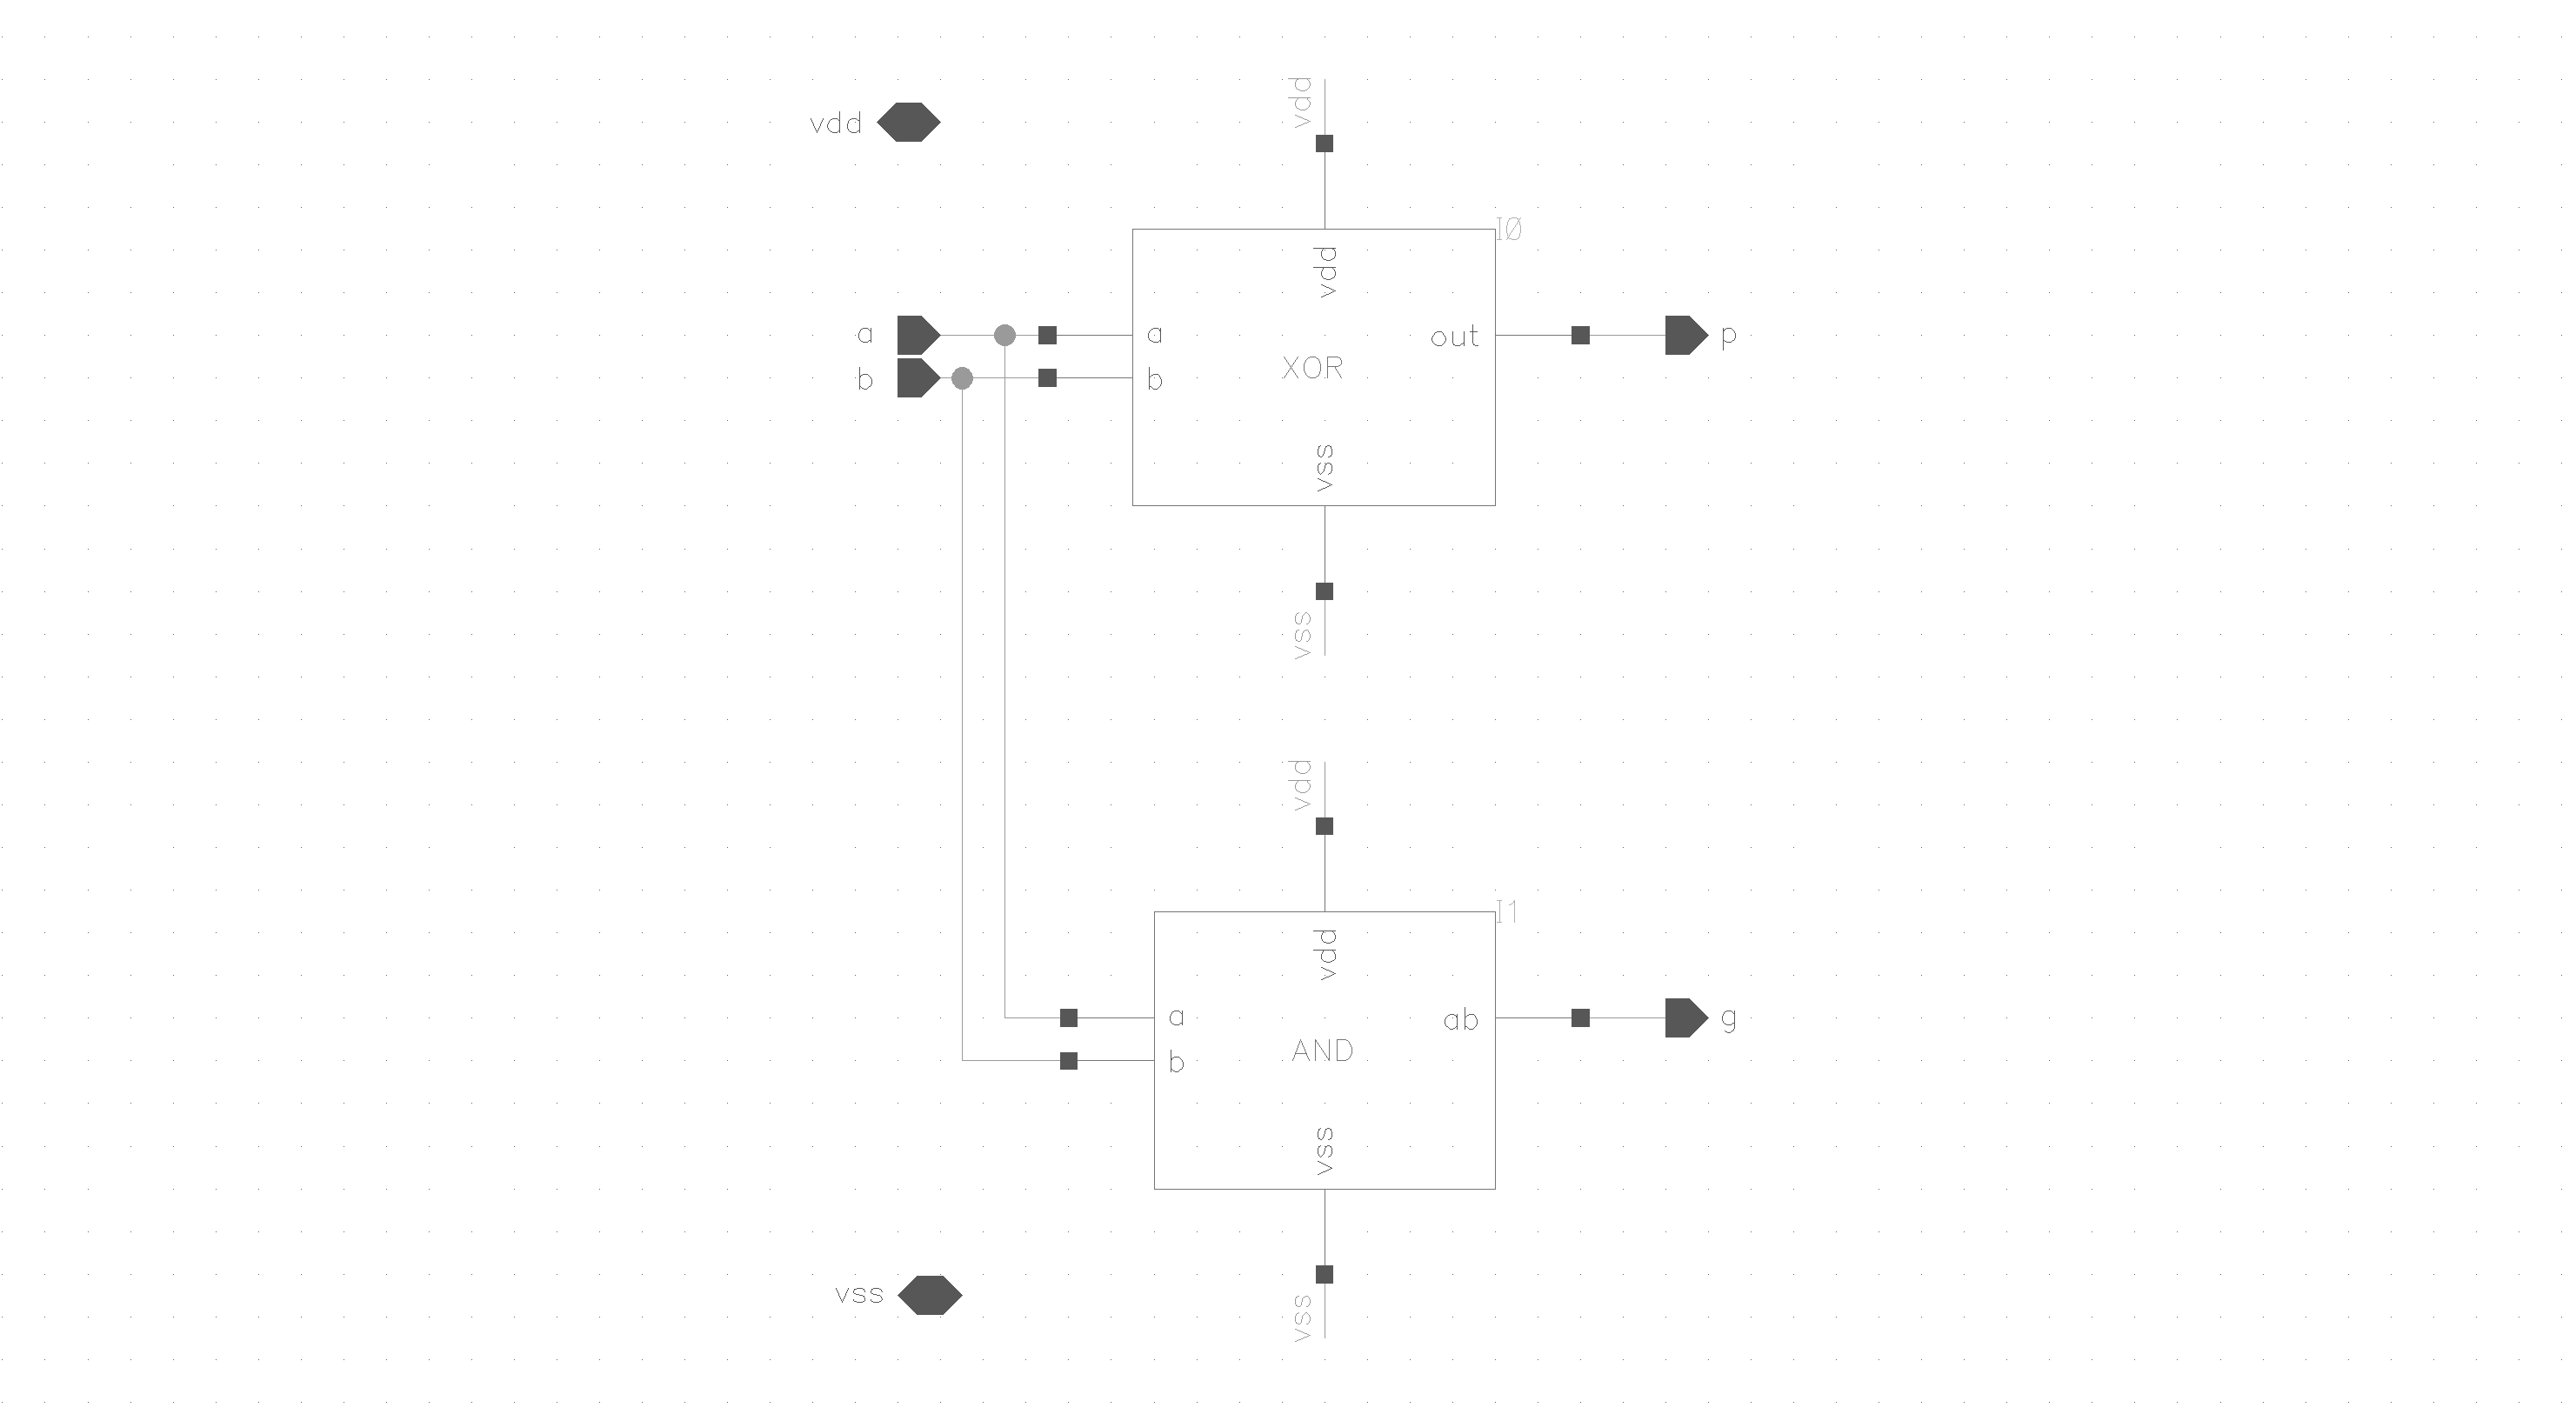
\includegraphics[clip,width=1.0\textwidth]{../figures/red}
  \caption{Figure shows whats inside the red block in the adder} \label{fig:red}
\end{figure}
\subsection{Comparator}

\begin{figure}[H]
  \centering
  \captionsetup{justification=centering}
  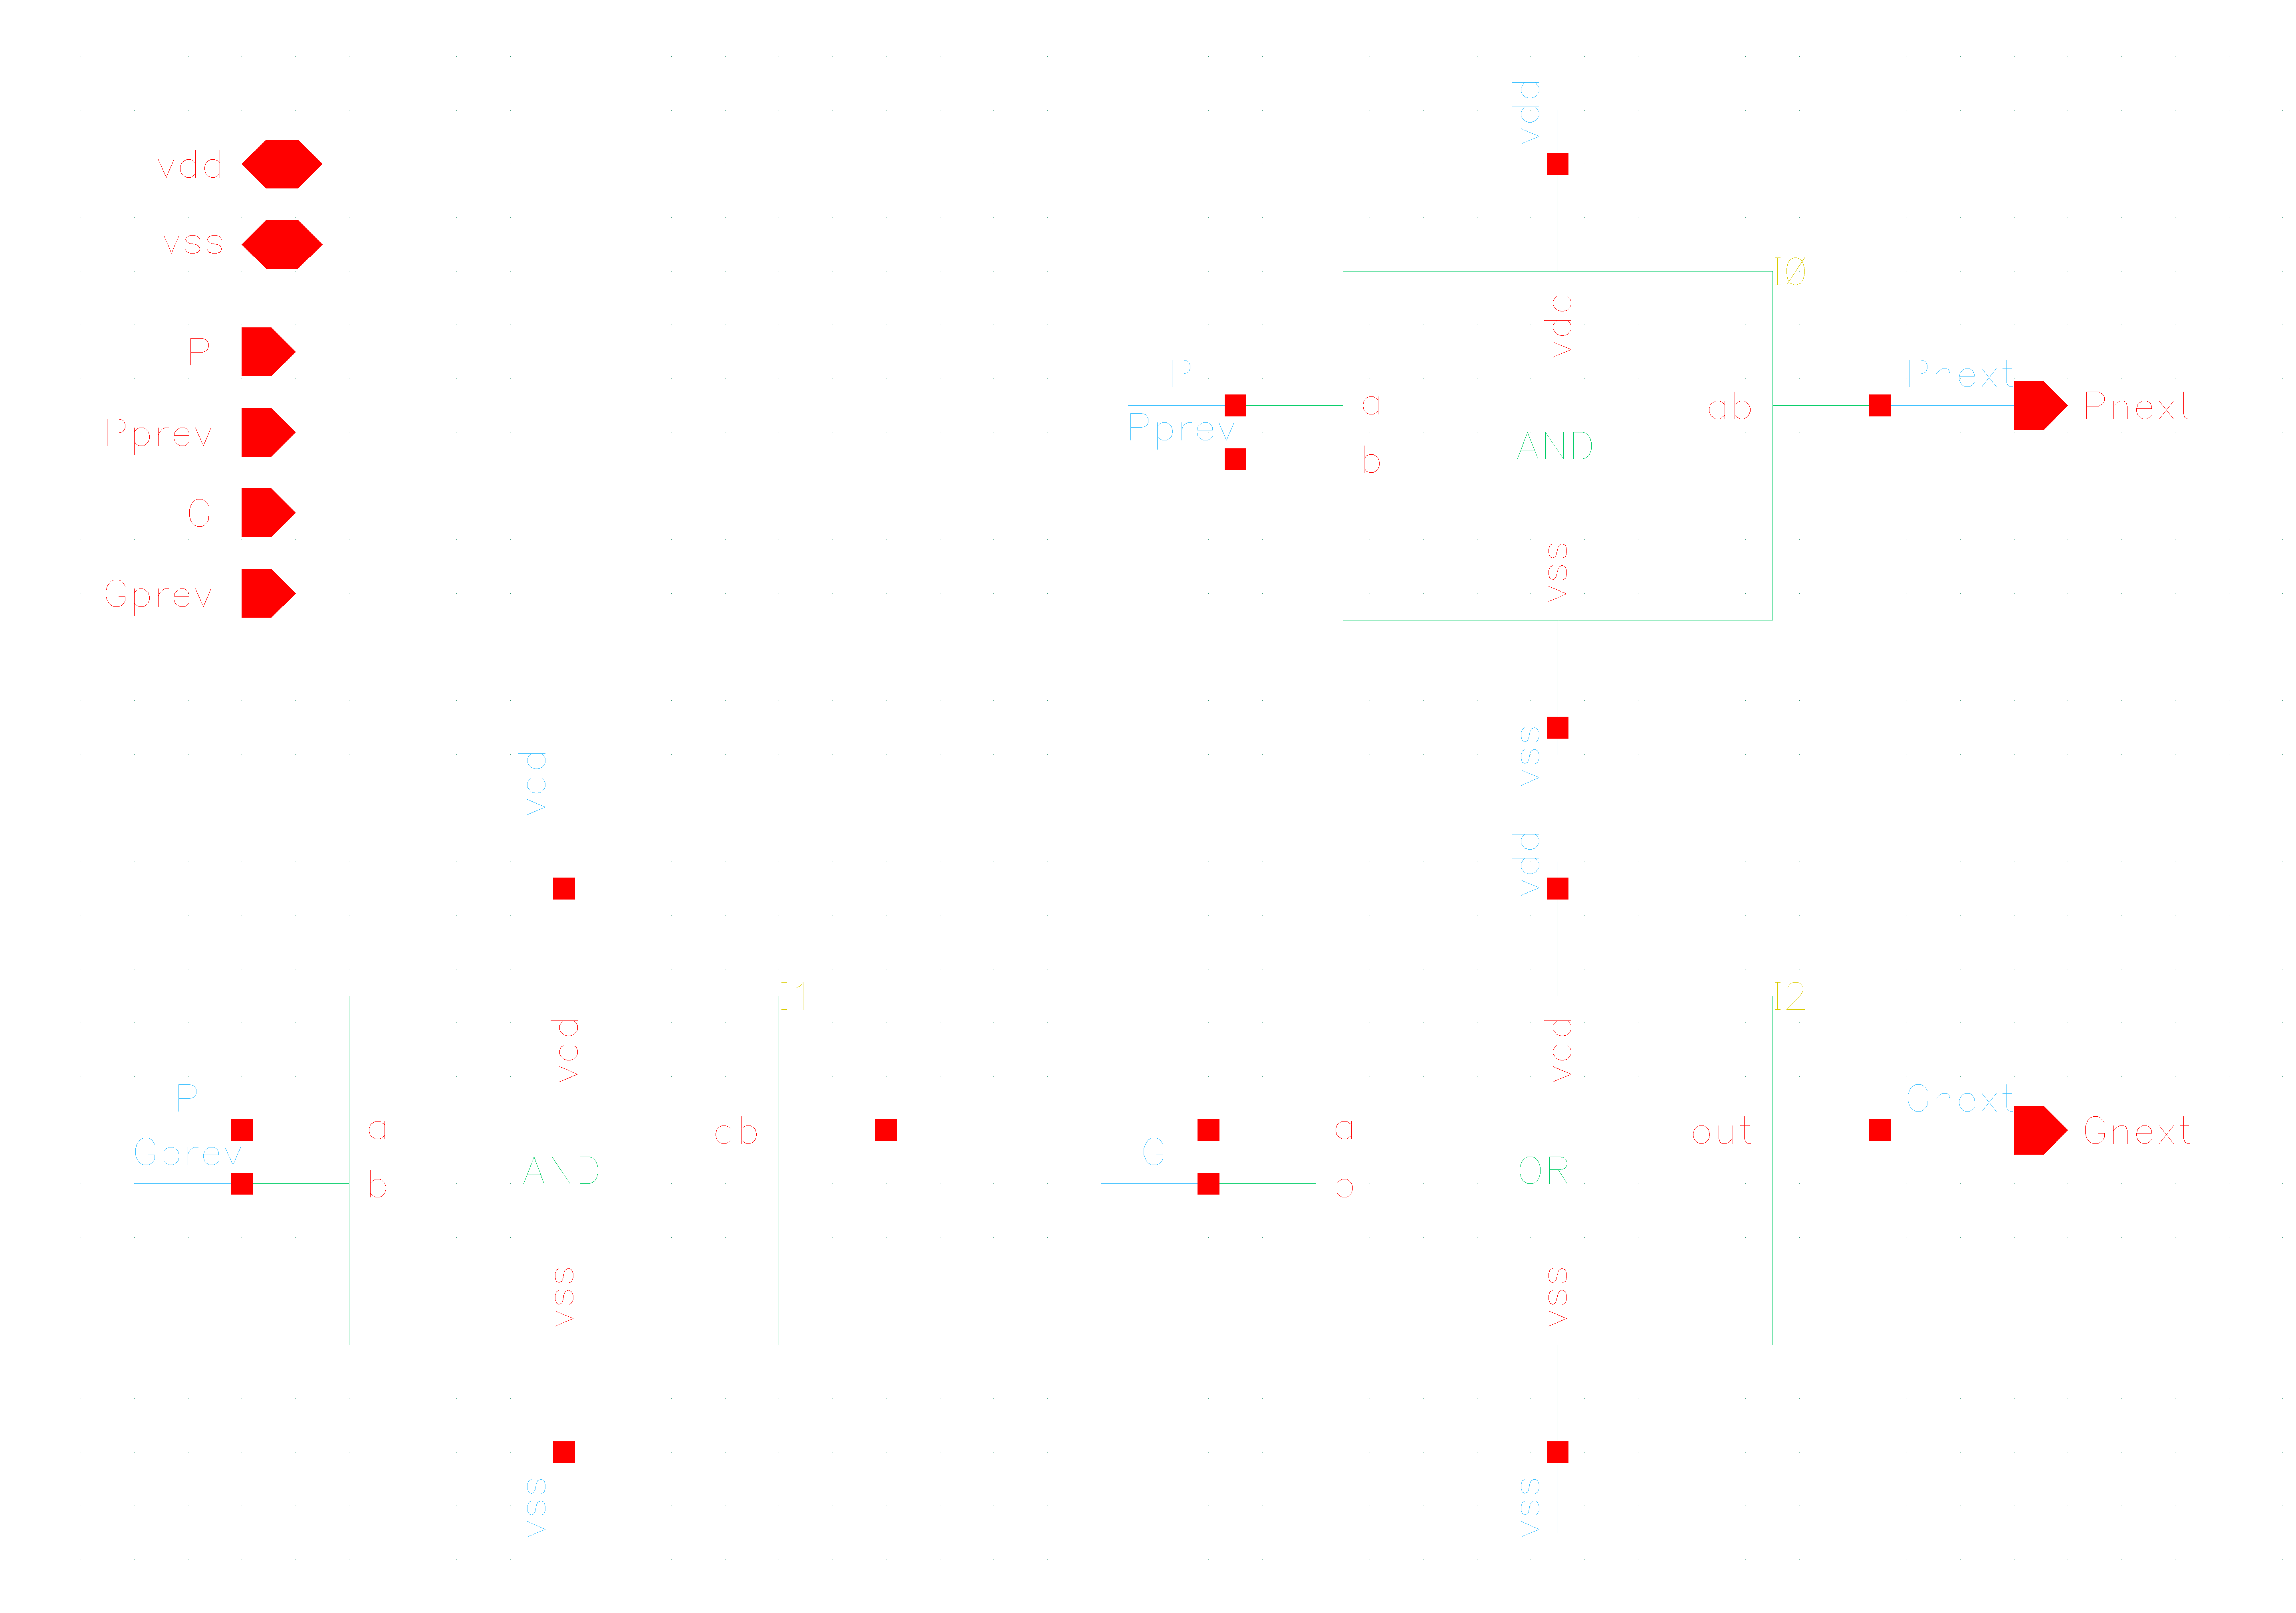
\includegraphics[clip,width=1.0\textwidth]{../figures/yellow}
  \caption{Figure shows whats inside the yellow block in the adder} \label{fig:yellow}
\end{figure}

\begin{figure}[H]
  \centering
  \captionsetup{justification=centering}
  \adjustbox{trim={0\width} {0\height} {0\width} {.4\height},clip}
  {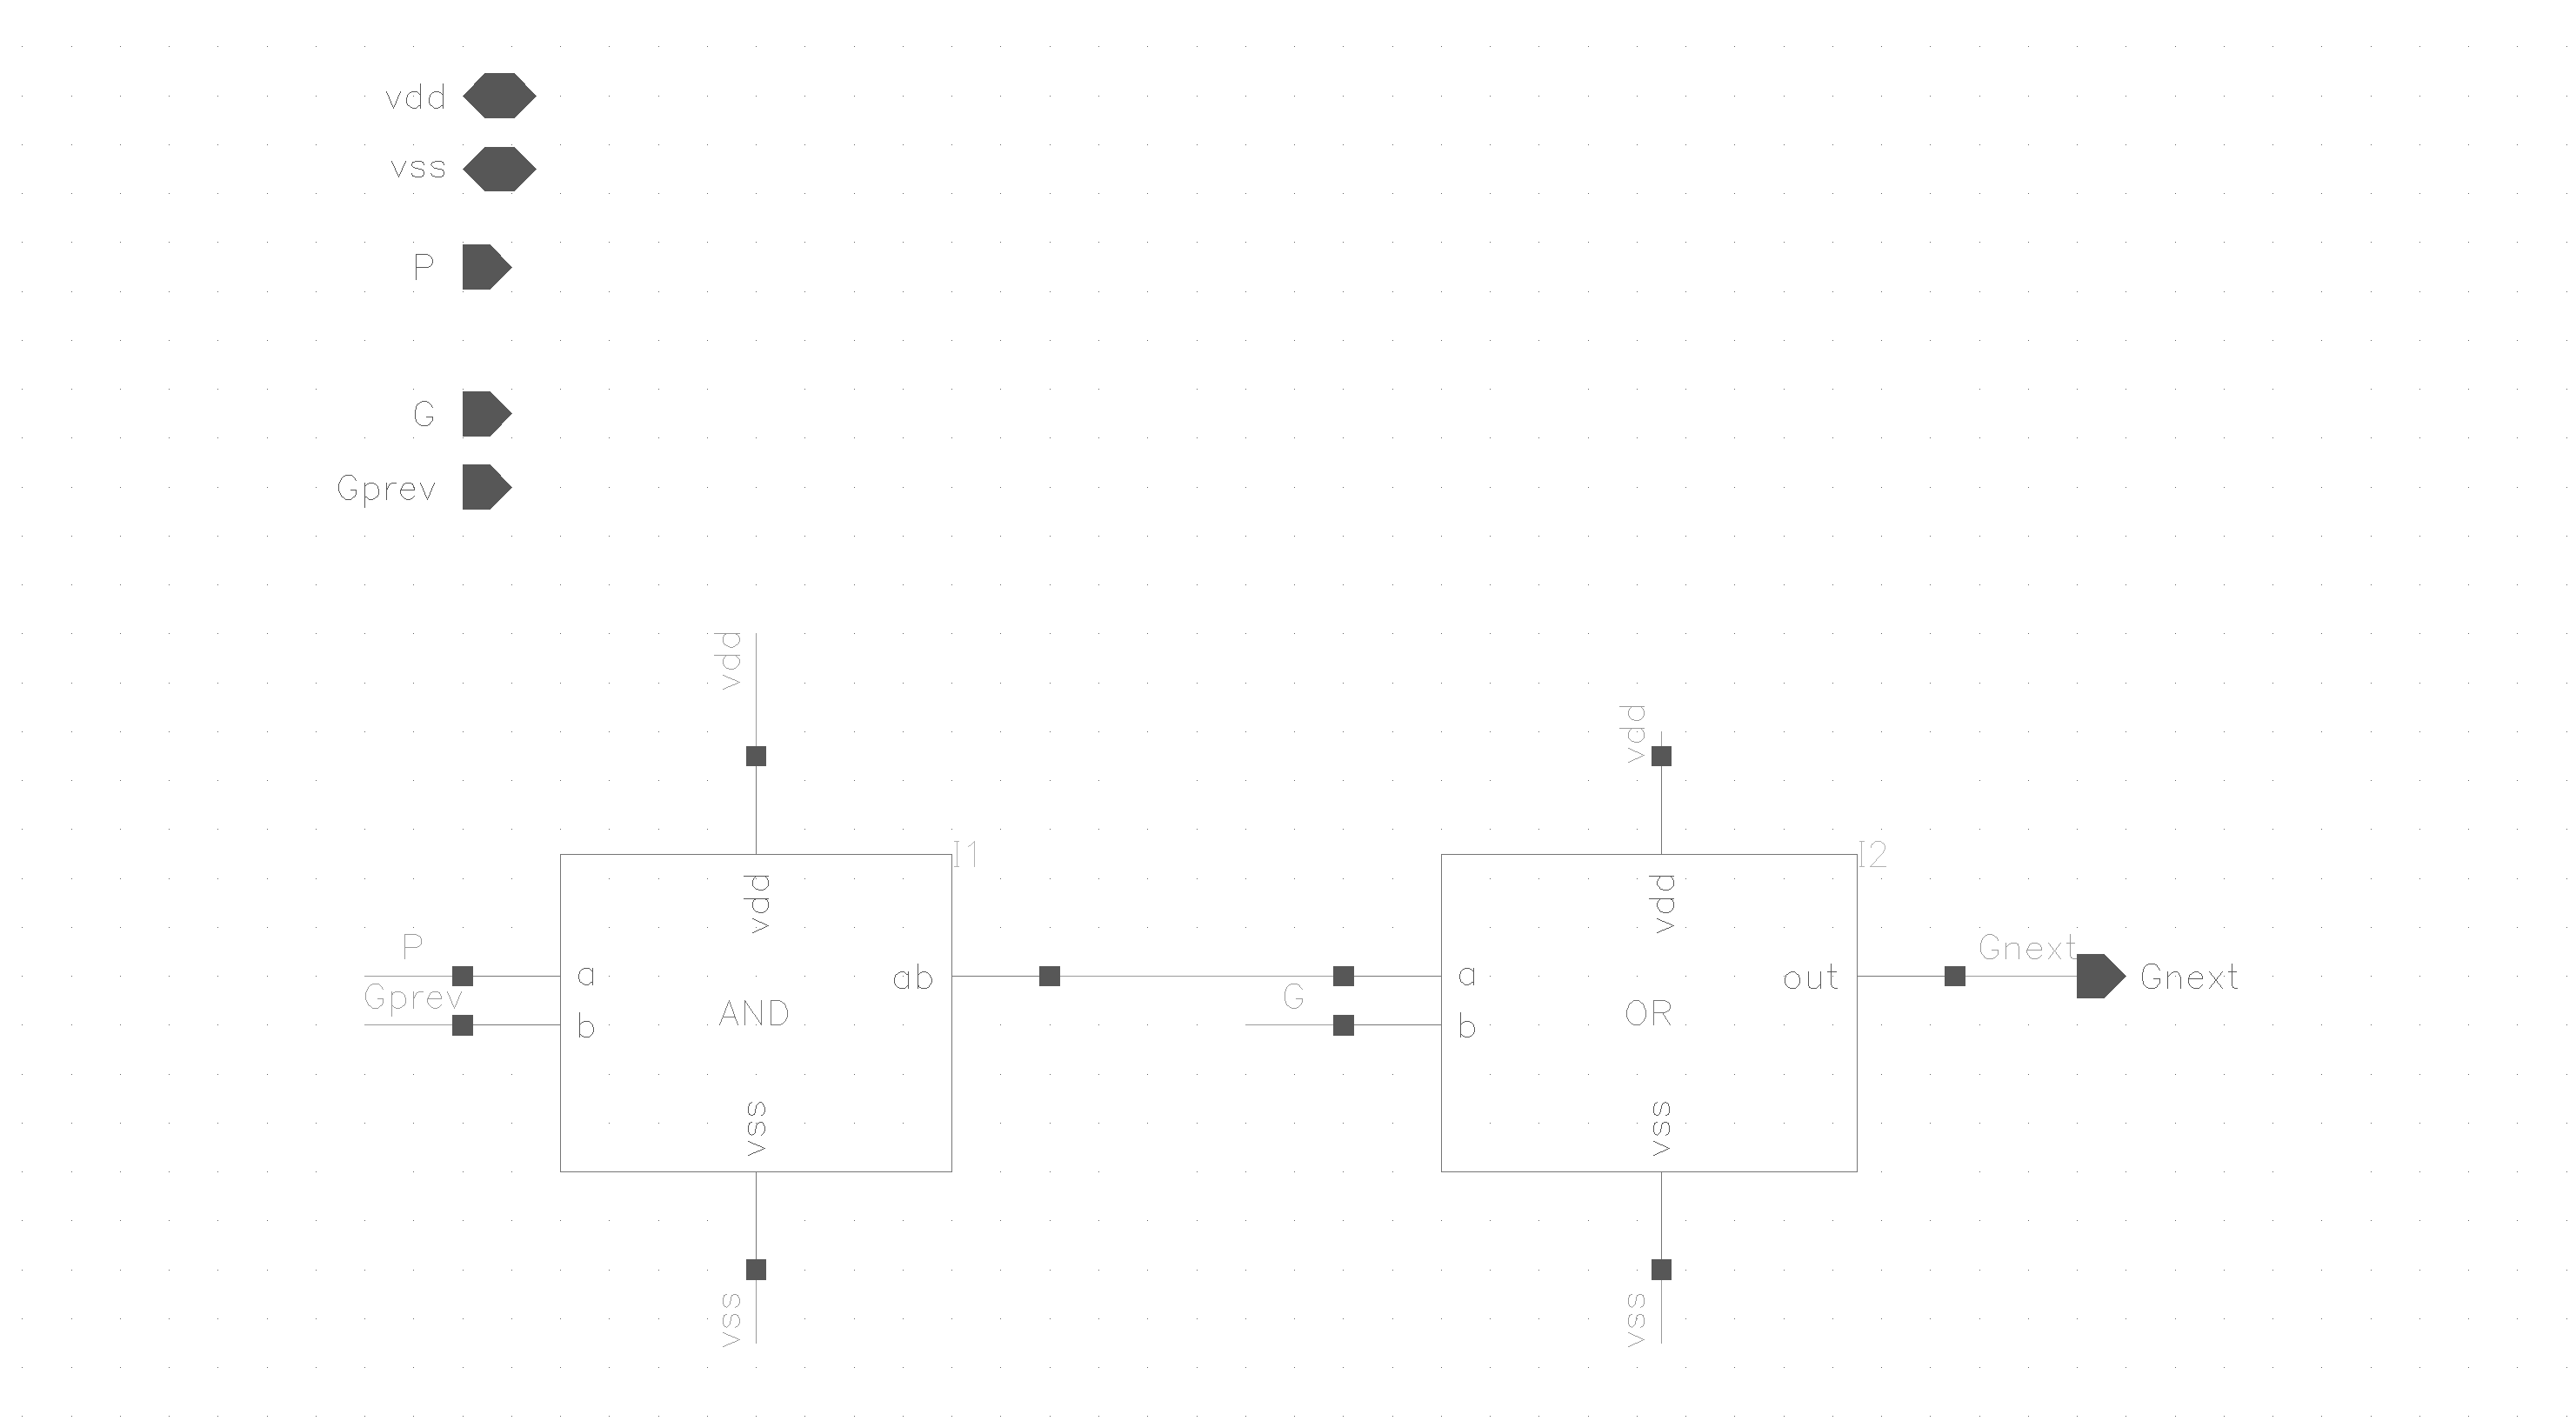
\includegraphics[width=1.0\textwidth]{../figures/yellow_carry}}
  \caption{Figure shows whats inside the yellow carry block in the adder} \label{fig:yellow_c}
\end{figure}

\begin{figure}[H]
  \centering
  \captionsetup{justification=centering}
  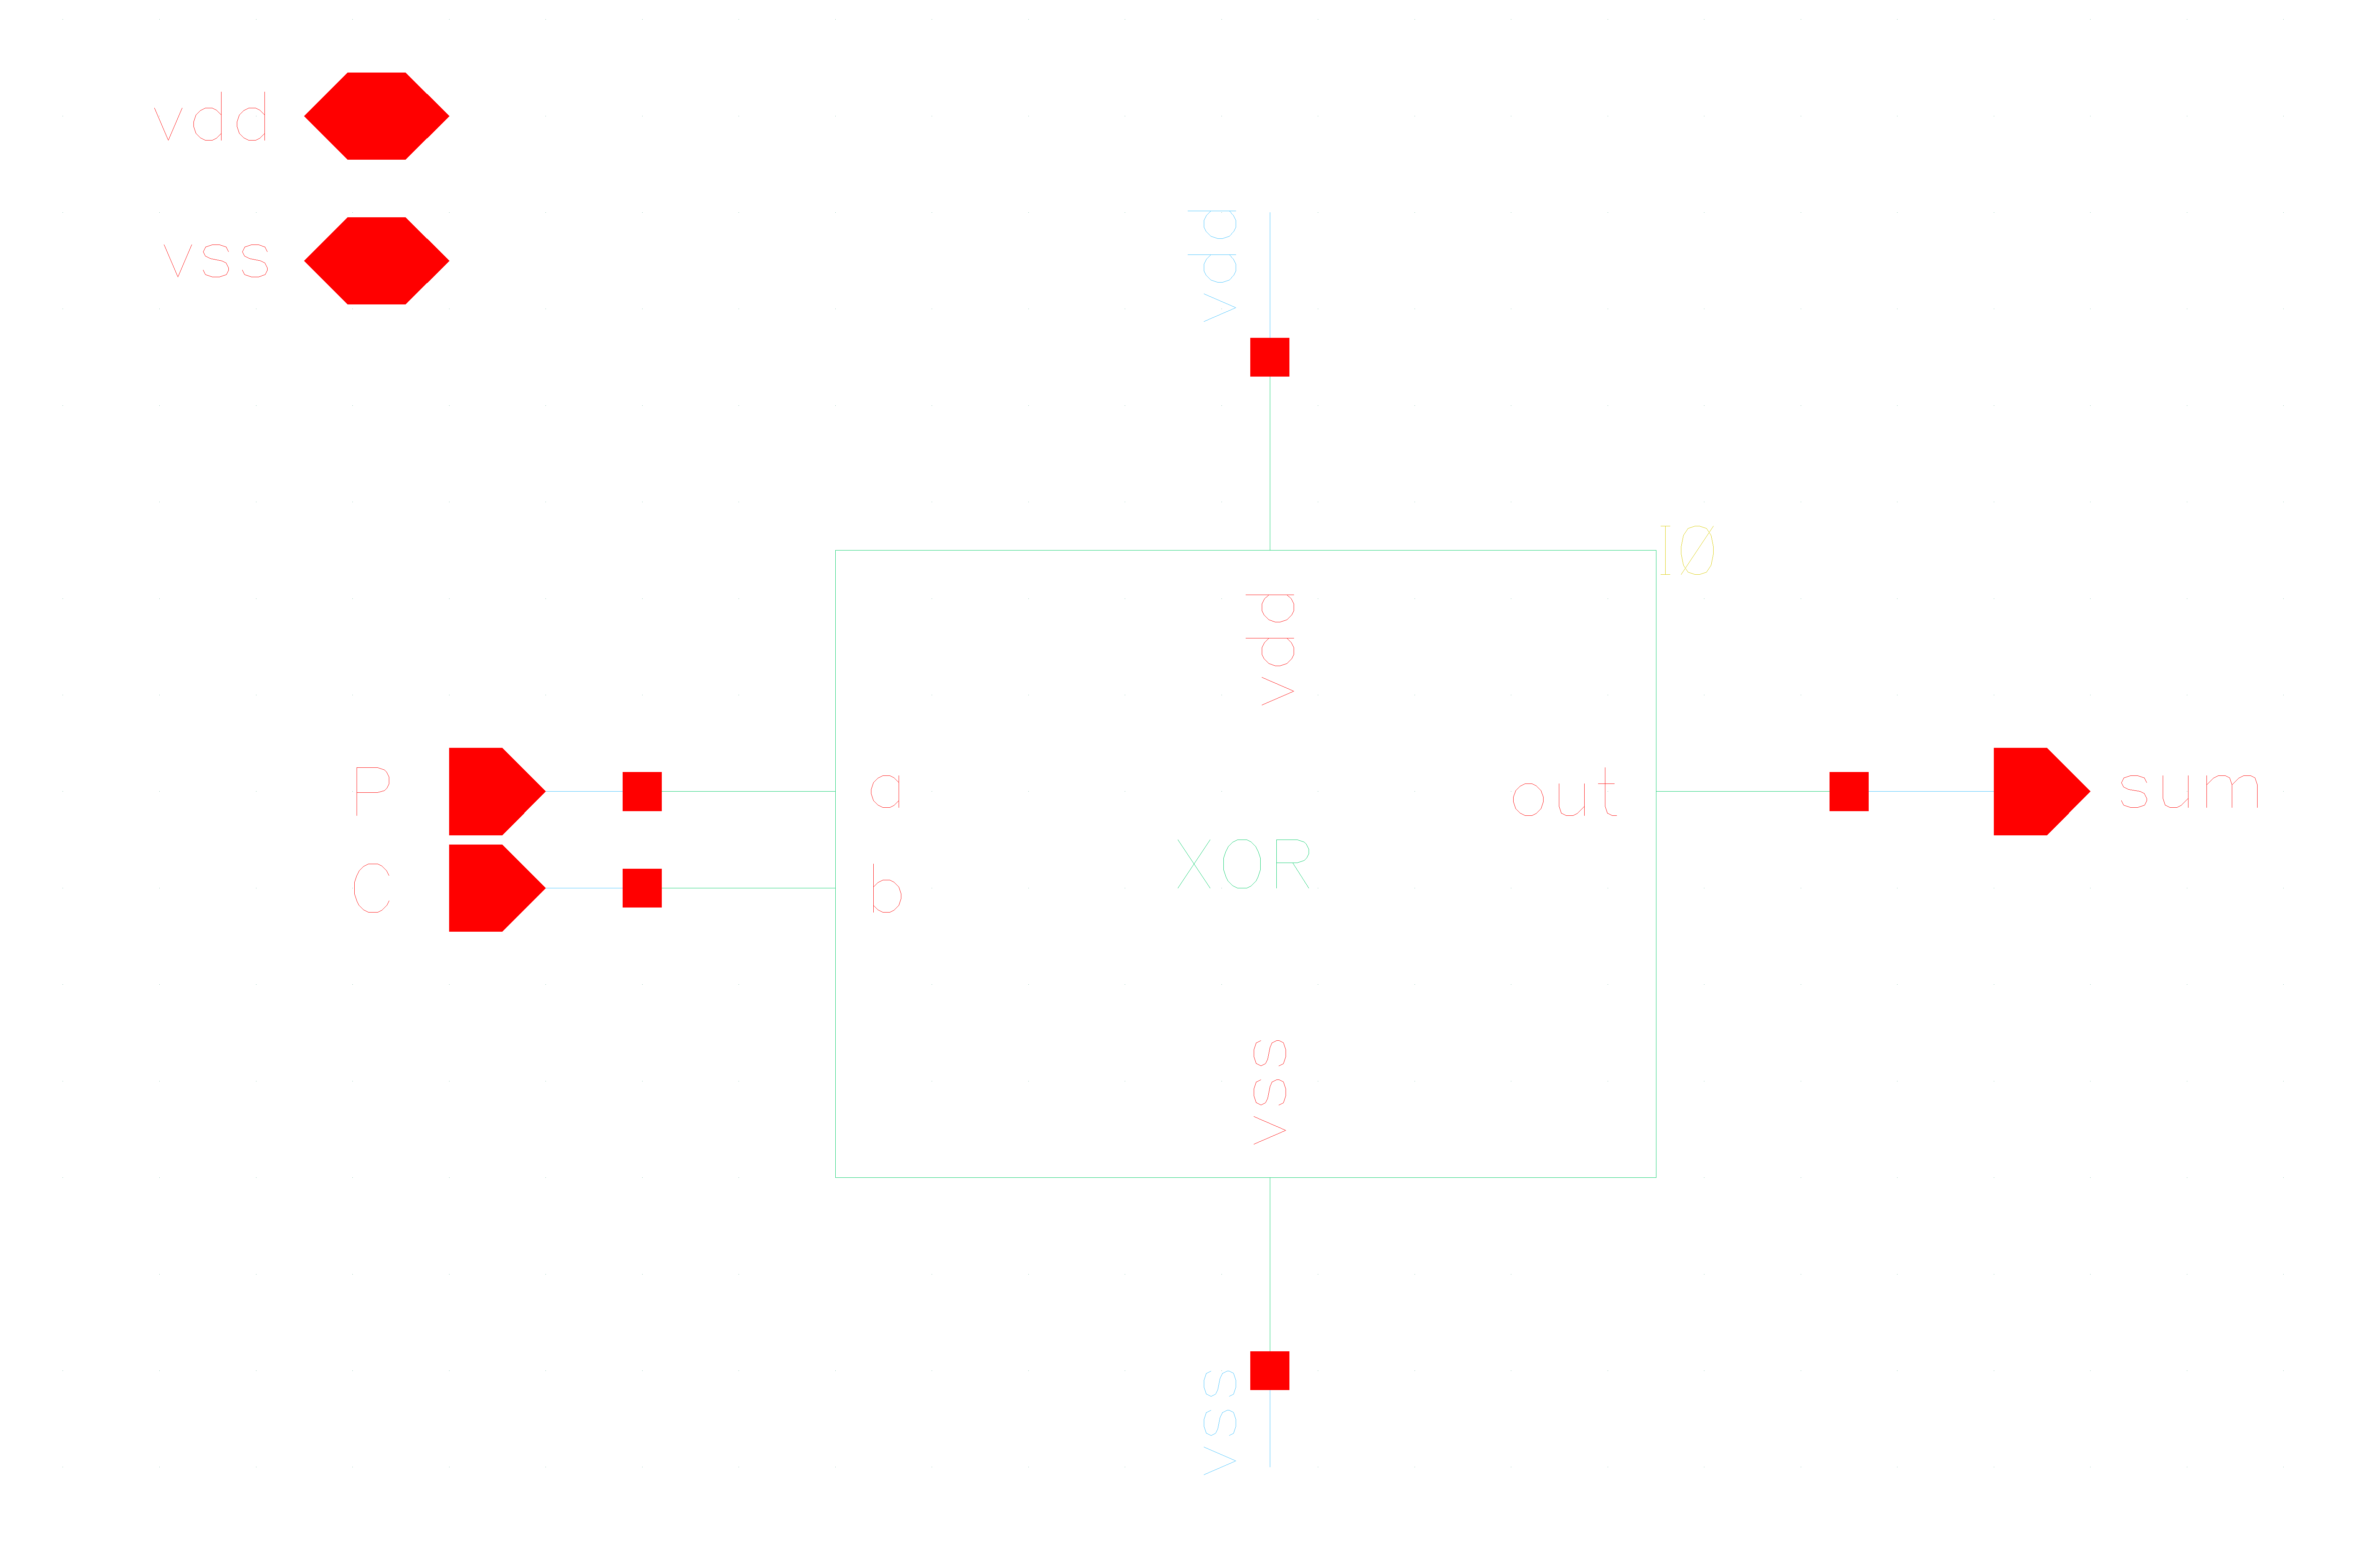
\includegraphics[clip,width=1.0\textwidth]{../figures/sum}
  \caption{Figure shows whats inside the sum block in the adder} \label{fig:sum}
\end{figure}
